

% Hey
\newpage
\section{Numerical Results}%
\label{sec:numerical_results}


On the numerical experiments shown on figures \ref{fig:man_conv},  the error norms is shown numerically that there exists a $C > 0$ such
that


\newpage
\subsection{Manufactured Solution}%
\label{sub:manufactured_solution}

All numerical experiments were carries out on the unit square with length $L$. A illustration of the triangulation can be seen on figure \ref{fig:sol_l1_m1_r1}.
The FEM software package used in the implementation was Gridap written in the Julia programming language \cite{verdugo22, julia17}.

\begin{equation}
    \label{eq:man_sol}
u\left( x; L,m,r \right) = \cos\left(  m\cdot \frac{2\pi}{L}  x_{1}\right)  \cos \left(r\cdot  \frac{2\pi}{L} x_{2} \right) \quad \text{ on }   \Omega =  \left( 0,L  \right)^{2}
.\end{equation}
For convenience did we pick $\alpha = 1$ for all the numerical experiments. We define the error to have the form $e = u - u_{h}$ such that the $L^2$ norm is denoted as $\| e \|_{ L^{2}\left( \Omega  \right)   }^{  } $, $H^{1}\left( \Omega  \right) $
norm is denoted as $\| e \|_{ H^{1}\left( \Omega  \right)  }^{  } $ and lastly the energy norm  \eqref{eq:A_energy_norm} defined as $\| e \|_{ h }^{  } $  .

\begin{figure}[tbh!]
    \centering
    \includegraphics[width=0.5\textwidth]{figures/model/l_1.0_m_1_r_1n_30_grid.png}
    \caption{Example of mesh on $ \Omega =  \left( 0,1  \right)^{2}$ where $h=\frac{1}{2^{4}}$  }
    \label{fig:sol_l1_m1_r1}
\end{figure}



\subsubsection{First Example, $L=1$, $m=7$, $r=3$}%
\label{sub:second_example}

\begin{figure}[tbh!]
    \centering
    \includegraphics[width=0.5\textwidth]{figures/model/l_1.0_m_7_r_3n_100_sol.png}
    \caption{Illustration of the manufactured solution \eqref{eq:man_sol}   with the parameters $L=1$, $m=7$ and $r=3$ in $\Omega = (0,1)^2$}
    \label{fig:sol_l1_m7_r3}
\end{figure}

\begin{figure}
    \centering
    \begin{minipage}{.5\linewidth}
    \centering
    \subfloat[]{\label{fig:ex1_gamma:a}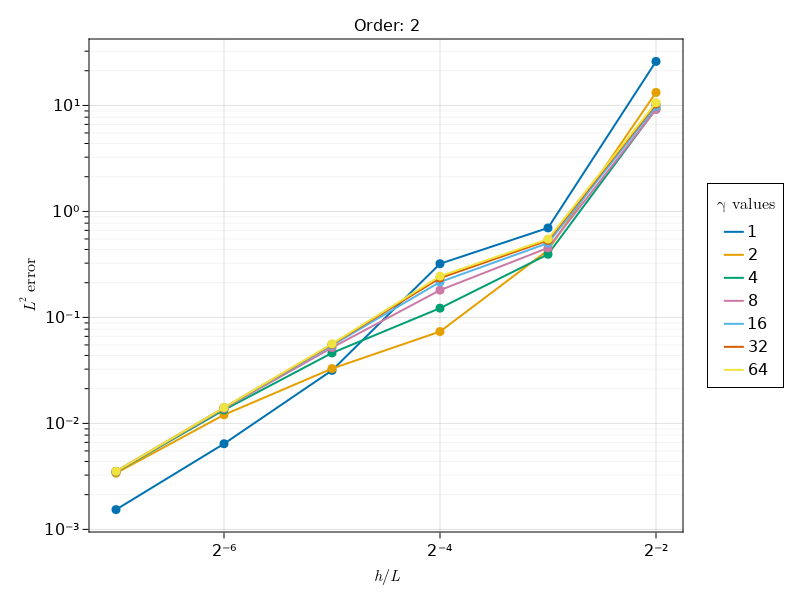
\includegraphics[scale=.25]{figures/convergence/L_1.0_m_7_r_3/gamma_analysis_order2.png}}
    \end{minipage}%
    \begin{minipage}{.5\linewidth}
    \centering
    \subfloat[]{\label{fig:ex1_gamma:b}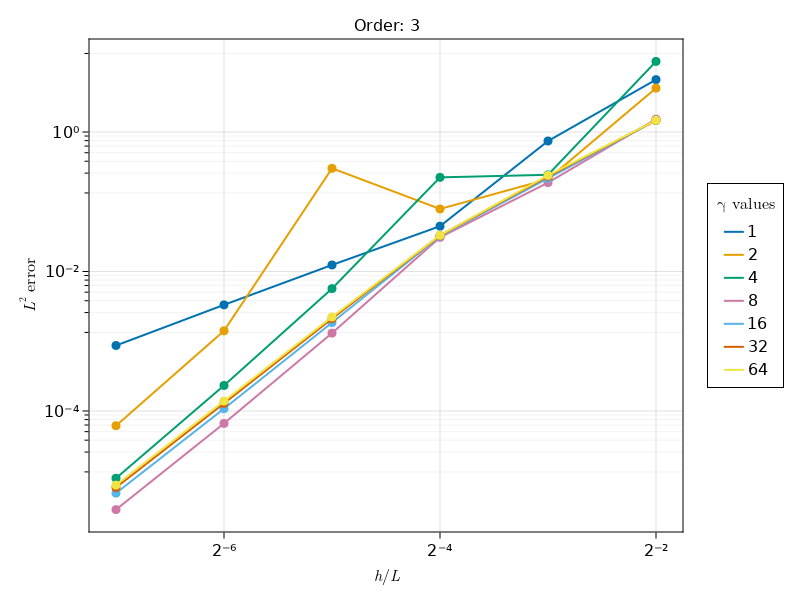
\includegraphics[scale=.25]{figures/convergence/L_1.0_m_7_r_3/gamma_analysis_order3.png}}
    \end{minipage}\par\medskip
    \centering
    \subfloat[]{\label{fig:ex1_gamma:c}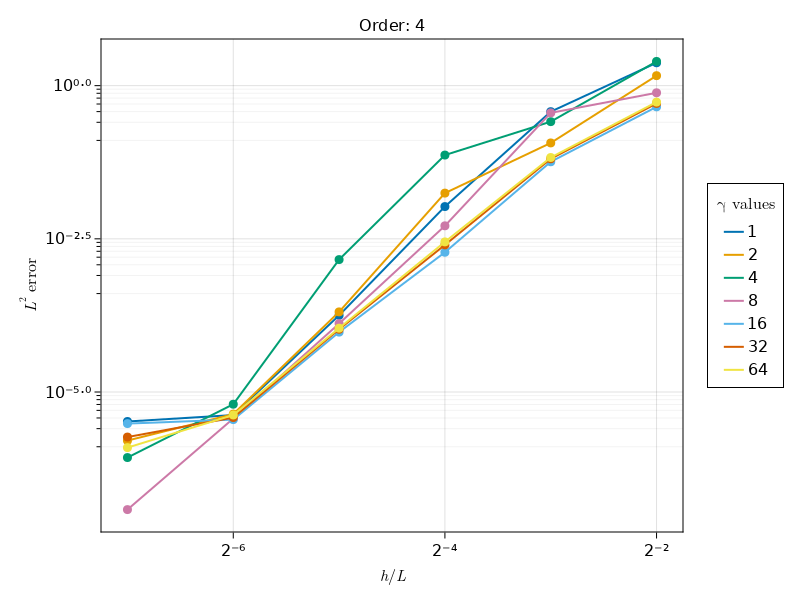
\includegraphics[scale=.25]{figures/convergence/L_1.0_m_7_r_3/gamma_analysis_order4.png}}
    \caption{ Example, $L=1$, $m=1$, $r=1$. $\gamma$ exploration with polynomials $\mathcal{P}_{k} $ with order $k$ . Figures \ref{fig:ex1_gamma:a}, \ref{fig:ex1_gamma:b} and \ref{fig:ex1_gamma:c} has respectively the order $k=2,3, 4$ .  }
    \label{fig:ex1_gamma}
\end{figure}


\begin{figure}
    \centering
    \begin{minipage}{.5\linewidth}
    \centering
    \subfloat[]{\label{fig:ex1_conv:a}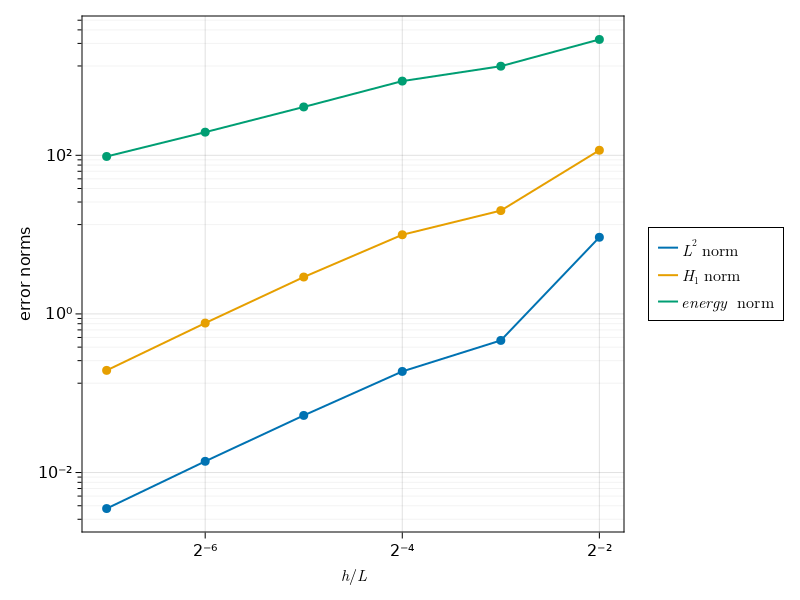
\includegraphics[scale=.25]{figures/convergence/L_1.0_m_7_r_3/conv_order_2_gamma_9.0.png}}
    \end{minipage}%
    \begin{minipage}{.5\linewidth}
    \centering
    \subfloat[]{\label{fig:ex1_conv:b}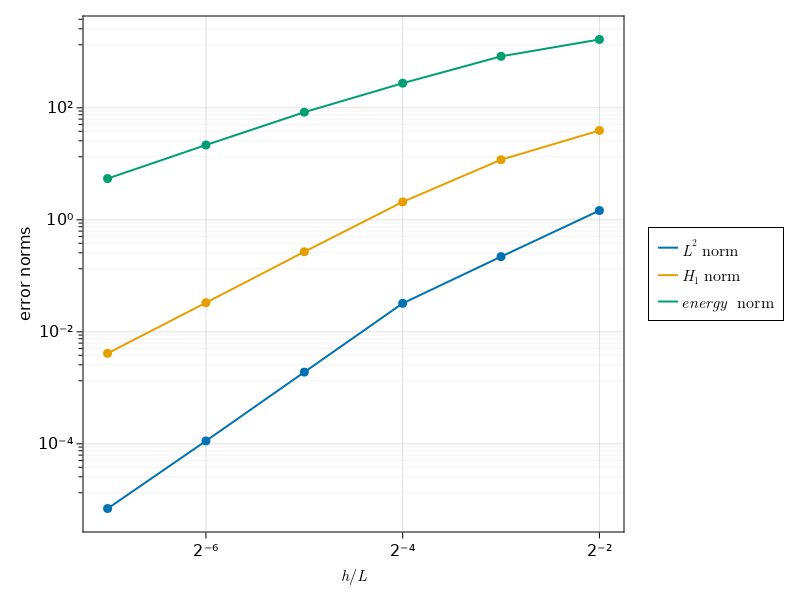
\includegraphics[scale=.25]{figures/convergence/L_1.0_m_7_r_3/conv_order_3_gamma_18.0.png}}
    \end{minipage}\par\medskip
    \centering
    \subfloat[]{\label{fig:ex1_conv:c}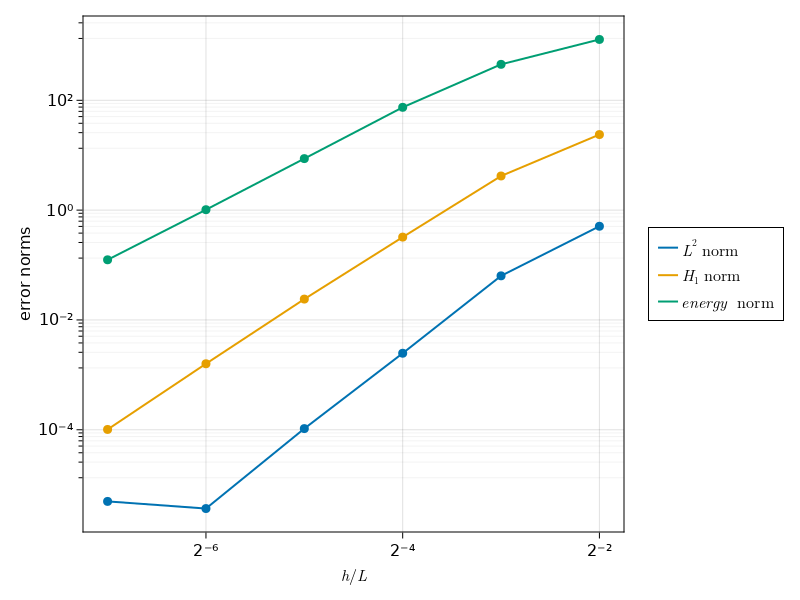
\includegraphics[scale=.25]{figures/convergence/L_1.0_m_7_r_3/conv_order_4_gamma_30.0.png}}
    \caption{ Example, $L=1$, $m=1$, $r=1$. Polynomials $\mathcal{P}_{k} $ with order $k$ . Figures \ref{fig:ex1_conv:a}, \ref{fig:ex1_conv:b} and \ref{fig:ex1_conv:c} has respectively the order $k=2,3, 4$ with penalty parameters $\gamma = 9,18,30 $.  }
    \label{fig:ex1_conv}
\end{figure}

Illustration can be seen on figure \ref{fig:ex1_conv} with convergence rate \ref{fig:ex1_conv}. The following table is

% Gammas for L=1
\begin{table}
  \caption{\label{tab:ex1_order2}  Order $k=2$ with $ \gamma = 9$.}
  \begin{tabular}{rrrrrrr}
    \hline\hline
    \textbf{$h/{L} $} & \textbf{$L^2$ norm} & \textbf{EOC} & \textbf{$H_1$ norm} & \textbf{EOC} & \textbf{energy norm} & \textbf{EOC} \\\hline
    $\frac{1}{4}$ & 9.253E+00 &  & 1.158E+02 &  & 2.888E+03 &  \\
    $\frac{1}{8}$ & 4.632E-01 & 4.320E+00 & 2.008E+01 & 2.527E+00 & 1.328E+03 & 1.120E+00 \\
    $\frac{1}{16}$ & 1.883E-01 & 1.299E+00 & 9.954E+00 & 1.013E+00 & 8.620E+02 & 6.238E-01 \\
    $\frac{1}{32}$ & 5.250E-02 & 1.842E+00 & 2.918E+00 & 1.770E+00 & 4.070E+02 & 1.083E+00 \\
    $\frac{1}{64}$ & 1.385E-02 & 1.922E+00 & 7.665E-01 & 1.929E+00 & 1.957E+02 & 1.056E+00 \\
    $\frac{1}{128}$ & 3.515E-03 & 1.979E+00 & 1.941E-01 & 1.981E+00 & 9.665E+01 & 1.018E+00 \\\hline\hline
  \end{tabular}
% \end{table}
% \begin{table}
  \caption{\label{tab:ex1_order3} Order $k=3$ with $ \gamma = 18$}
  \begin{tabular}{rrrrrrr}
    \hline\hline
    \textbf{$h/{L} $} & \textbf{$L^2$ norm} & \textbf{EOC} & \textbf{$H_1$ norm} & \textbf{EOC} & \textbf{energy norm} & \textbf{EOC} \\\hline
    $\frac{1}{4}$ & 1.466E+00 &  & 3.942E+01 &  & 1.664E+03 &  \\
    $\frac{1}{8}$ & 2.203E-01 & 2.735E+00 & 1.184E+01 & 1.736E+00 & 8.318E+02 & 1.000E+00 \\
    $\frac{1}{16}$ & 3.231E-02 & 2.769E+00 & 2.092E+00 & 2.500E+00 & 2.758E+02 & 1.593E+00 \\
    $\frac{1}{32}$ & 1.910E-03 & 4.081E+00 & 2.690E-01 & 2.959E+00 & 8.364E+01 & 1.721E+00 \\
    $\frac{1}{64}$ & 1.127E-04 & 4.083E+00 & 3.316E-02 & 3.020E+00 & 2.171E+01 & 1.946E+00 \\
    $\frac{1}{128}$ & 6.988E-06 & 4.011E+00 & 4.131E-03 & 3.005E+00 & 5.461E+00 & 1.991E+00 \\\hline\hline
  \end{tabular}
% \end{table}
  \caption{\label{tab:ex1_order4}Order $k=4$ with $ \gamma = 30$}
% \begin{table}
  \begin{tabular}{rrrrrrr}
    \hline\hline
    \textbf{$h/{L} $} & \textbf{$L^2$ norm} & \textbf{EOC} & \textbf{$H_1$ norm} & \textbf{EOC} & \textbf{energy norm} & \textbf{EOC} \\\hline
    $\frac{1}{4}$ & 5.083E-01 &  & 2.377E+01 &  & 1.282E+03 &  \\
    $\frac{1}{8}$ & 6.355E-02 & 3.000E+00 & 4.185E+00 & 2.506E+00 & 4.516E+02 & 1.505E+00 \\
    $\frac{1}{16}$ & 2.475E-03 & 4.682E+00 & 3.223E-01 & 3.699E+00 & 7.450E+01 & 2.600E+00 \\
    $\frac{1}{32}$ & 1.050E-04 & 4.559E+00 & 2.398E-02 & 3.749E+00 & 8.670E+00 & 3.103E+00 \\
    $\frac{1}{64}$ & 3.675E-06 & 4.837E+00 & 1.593E-03 & 3.912E+00 & 1.018E+00 & 3.090E+00 \\
    $\frac{1}{128}$ & 4.958E-06 & -4.319E-01 & 1.013E-04 & 3.974E+00 & 1.246E-01 & 3.031E+00 \\\hline\hline
  \end{tabular}
\end{table}


\subsubsection{Second Example, $L=2 \pi $, $m=1$, $r=1$}%
\label{sub:first_example}

\begin{figure}[tbh!]
    \centering
    \includegraphics[width=0.5\textwidth]{figures/model/l_6.28_m_1_r_1n_100_sol.png}
    \caption{Illustration of the manufactured solution \eqref{eq:man_sol}   with the parameters $L=2\pi$, $m=1$ and $r=1$ in $\Omega = (0,2\pi)^2$}
    \label{fig:sol_l2pi_m1_r1}
\end{figure}

Illustration can be seen on figure \ref{fig:sol_l2pi_m1_r1} with gamma convergence plots on \ref{fig:ex2_gamma}. Also some convergence analysis on specified gammas on of \ref{fig:ex2_conv}.

\begin{figure}
    \centering
    \begin{minipage}{.5\linewidth}
    \centering
    \subfloat[]{\label{fig:ex2_gamma:a}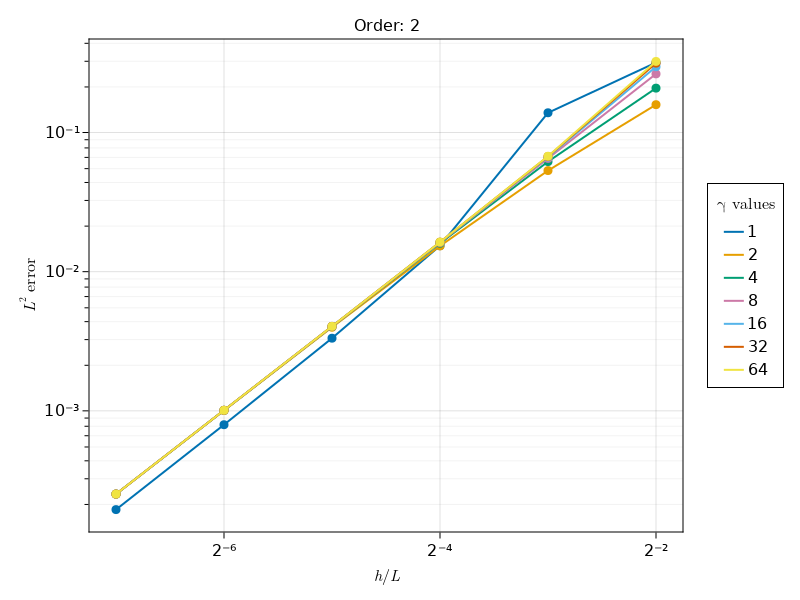
\includegraphics[scale=.25]{figures/convergence/L_6.28_m_1_r_1/gamma_analysis_order2.png}}
    \end{minipage}%
    \begin{minipage}{.5\linewidth}
    \centering
    \subfloat[]{\label{fig:ex2_gamma:b}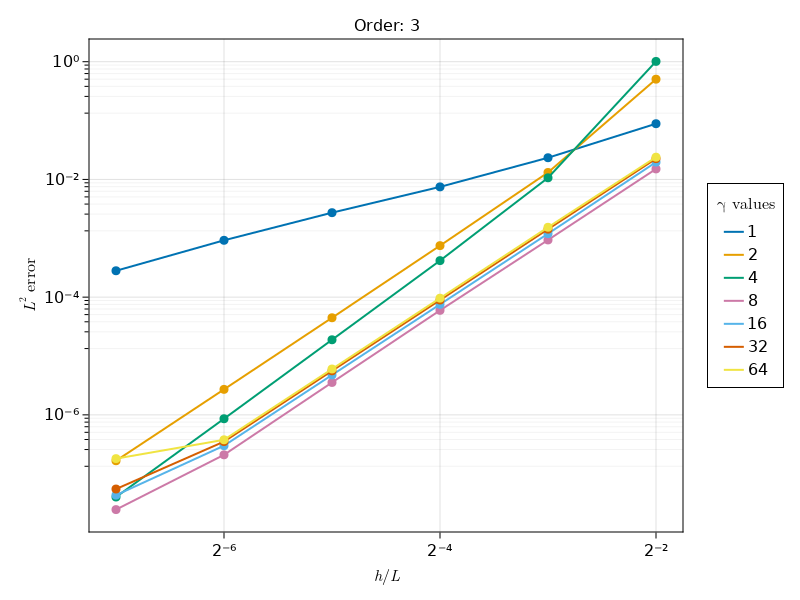
\includegraphics[scale=.25]{figures/convergence/L_6.28_m_1_r_1/gamma_analysis_order3.png}}
    \end{minipage}\par\medskip
    \centering
    \subfloat[]{\label{fig:ex2_gamma:c}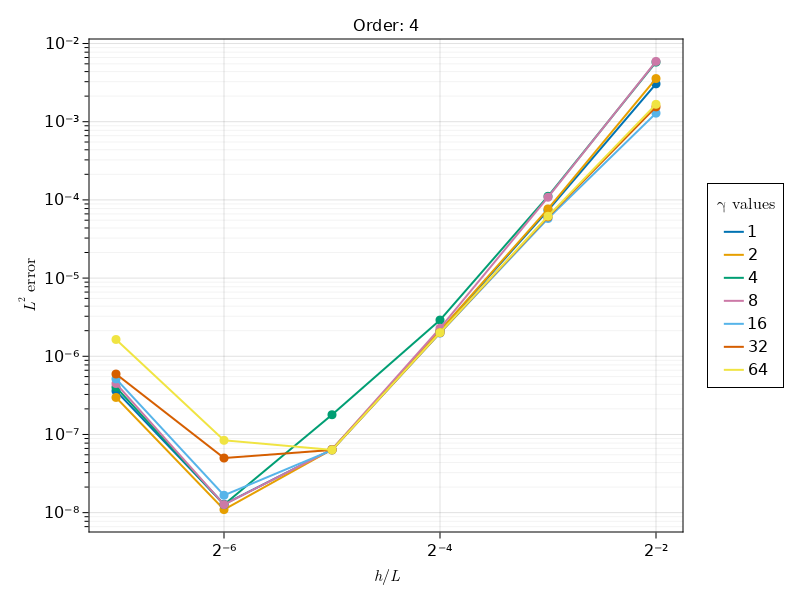
\includegraphics[scale=.25]{figures/convergence/L_6.28_m_1_r_1/gamma_analysis_order4.png}}
    \caption{ Example, $L=1$, $m=1$, $r=1$. $\gamma$ exploration with polynomials $\mathcal{P}_{k} $ with order $k$ . Figures \ref{fig:ex2_gamma:a}, \ref{fig:ex2_gamma:b} and \ref{fig:ex2_gamma:c} has respectively the order $k=2,3, 4$ .  }
    \label{fig:ex2_gamma}
\end{figure}

\begin{figure}
    \centering
    \begin{minipage}{.5\linewidth}
    \centering
    \subfloat[]{\label{fig:ex2_conv:a}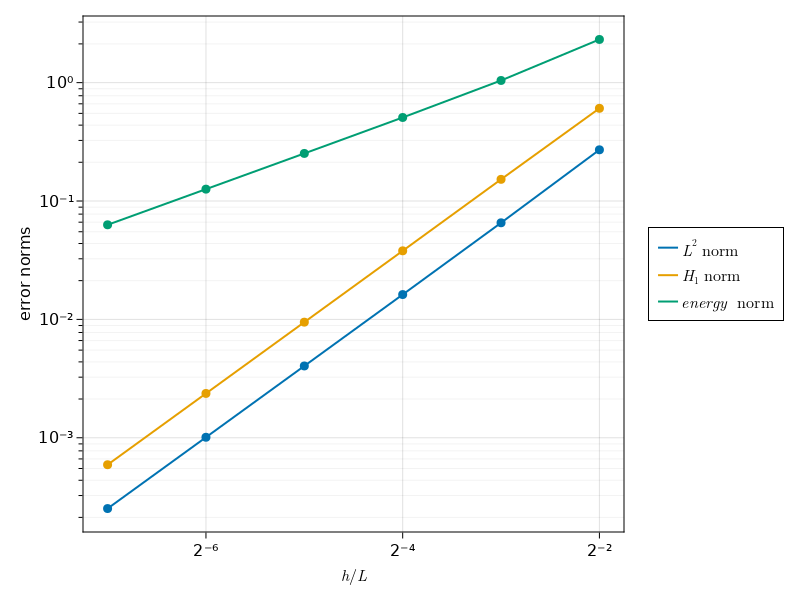
\includegraphics[scale=.2]{figures/convergence/L_6.28_m_1_r_1/conv_order_2_gamma_9.0.png}}
    \end{minipage}%
    \begin{minipage}{.5\linewidth}
    \centering
    \subfloat[]{\label{fig:ex2_conv:b}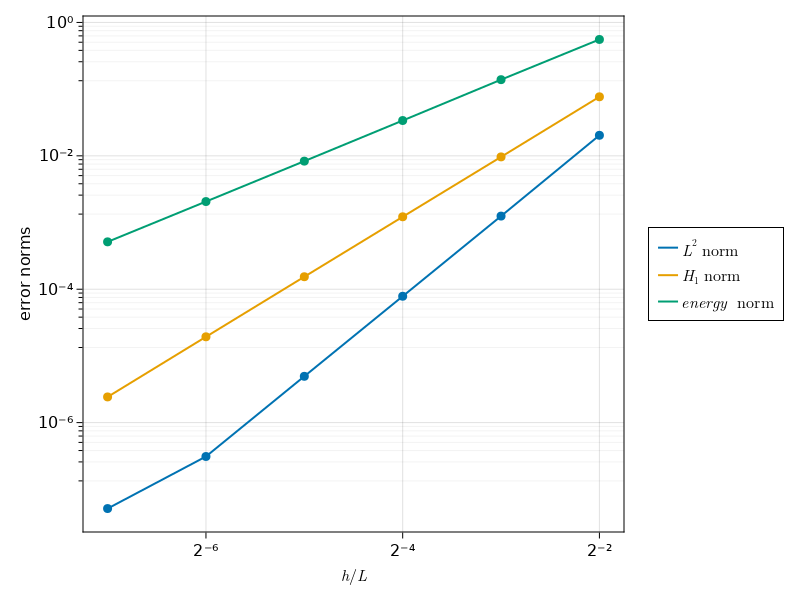
\includegraphics[scale=.2]{figures/convergence/L_6.28_m_1_r_1/conv_order_3_gamma_18.0.png}}
    \end{minipage}\par\medskip
    \centering
    \subfloat[]{\label{fig:ex2_conv:c}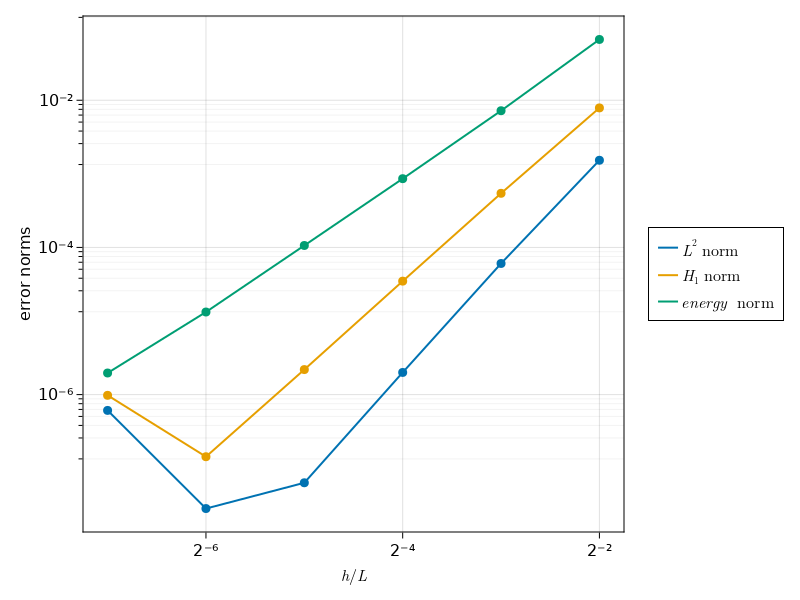
\includegraphics[scale=.2]{figures/convergence/L_6.28_m_1_r_1/conv_order_4_gamma_30.0.png}}
    \caption{ Example, $L=1$, $m=1$, $r=1$. Polynomials $\mathcal{P}_{k} $ with order $k$ . Figures \ref{fig:ex2_conv:a}, \ref{fig:ex2_conv:b} and \ref{fig:ex2_conv:c} has respectively the order $k=2,3, 4$ with penalty parameters $\gamma = 9,18,30 $.  }
    \label{fig:ex2_conv}
\end{figure}



% Gammas for L=2pi
\begin{table}
  \caption{\label{tab:ex2_order2} Order $k=2$ with $ \gamma = 9$}
  \begin{tabular}{rrrrrrr}
    \hline\hline
    \textbf{$h/{L} $} & \textbf{$L^2$ norm} & \textbf{EOC} & \textbf{$H_1$ norm} & \textbf{EOC} & \textbf{energy norm} & \textbf{EOC} \\\hline
    $\frac{1}{4}$ & 2.708E-01 &  & 6.068E-01 &  & 2.316E+00 &  \\
    $\frac{1}{8}$ & 6.547E-02 & 2.048E+00 & 1.524E-01 & 1.993E+00 & 1.043E+00 & 1.151E+00 \\
    $\frac{1}{16}$ & 1.621E-02 & 2.014E+00 & 3.796E-02 & 2.006E+00 & 5.078E-01 & 1.039E+00 \\
    $\frac{1}{32}$ & 4.041E-03 & 2.004E+00 & 9.475E-03 & 2.002E+00 & 2.523E-01 & 1.009E+00 \\
    $\frac{1}{64}$ & 1.010E-03 & 2.001E+00 & 2.367E-03 & 2.001E+00 & 1.260E-01 & 1.002E+00 \\
    $\frac{1}{128}$ & 2.524E-04 & 2.000E+00 & 5.918E-04 & 2.000E+00 & 6.296E-02 & 1.001E+00 \\\hline\hline
  \end{tabular}
% \end{table}

% \begin{table}
  \caption{\label{tab:ex2_order3} Order $k=3$ with $ \gamma = 18$.}
  \begin{tabular}{rrrrrrr}
    \hline\hline
    \textbf{$h/{L} $} & \textbf{$L^2$ norm} & \textbf{EOC} & \textbf{$H_1$ norm} & \textbf{EOC} & \textbf{energy norm} & \textbf{EOC} \\\hline
    $\frac{1}{4}$ & 2.032E-02 &  & 7.678E-02 &  & 5.558E-01 &  \\
    $\frac{1}{8}$ & 1.249E-03 & 4.024E+00 & 9.639E-03 & 2.994E+00 & 1.387E-01 & 2.003E+00 \\
    $\frac{1}{16}$ & 7.845E-05 & 3.993E+00 & 1.219E-03 & 2.983E+00 & 3.385E-02 & 2.035E+00 \\
    $\frac{1}{32}$ & 4.946E-06 & 3.987E+00 & 1.539E-04 & 2.986E+00 & 8.327E-03 & 2.023E+00 \\
    $\frac{1}{64}$ & 3.104E-07 & 3.994E+00 & 1.935E-05 & 2.992E+00 & 2.063E-03 & 2.013E+00 \\
    $\frac{1}{128}$ & 5.147E-08 & 2.592E+00 & 2.427E-06 & 2.995E+00 & 5.134E-04 & 2.007E+00 \\\hline\hline
  \end{tabular}
% \end{table}

% \begin{table}
  \caption{\label{tab:ex2_order4} Order $k=4$ with $ \gamma = 30$}
  \begin{tabular}{rrrrrrr}
    \hline\hline
    \textbf{$h/{L} $} & \textbf{$L^2$ norm} & \textbf{EOC} & \textbf{$H_1$ norm} & \textbf{EOC} & \textbf{energy norm} & \textbf{EOC} \\\hline
    $\frac{1}{4}$ & 1.529E-03 &  & 7.869E-03 &  & 6.700E-02 &  \\
    $\frac{1}{8}$ & 6.050E-05 & 4.660E+00 & 5.437E-04 & 3.855E+00 & 7.205E-03 & 3.217E+00 \\
    $\frac{1}{16}$ & 2.000E-06 & 4.919E+00 & 3.482E-05 & 3.965E+00 & 8.594E-04 & 3.068E+00 \\
    $\frac{1}{32}$ & 6.335E-08 & 4.980E+00 & 2.189E-06 & 3.992E+00 & 1.063E-04 & 3.016E+00 \\
    $\frac{1}{64}$ & 2.828E-08 & 1.164E+00 & 1.432E-07 & 3.934E+00 & 1.325E-05 & 3.003E+00 \\
    $\frac{1}{128}$ & 6.097E-07 & -4.430E+00 & 9.776E-07 & -2.772E+00 & 1.965E-06 & 2.753E+00 \\\hline\hline
  \end{tabular}
\end{table}


